\section{Design principles for ML}


\begin{figure}[H]
    \centering
    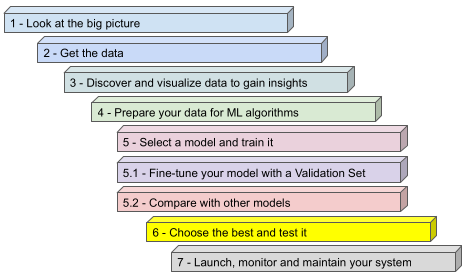
\includegraphics[width=0.6\linewidth]{/home/dmo/git/appunti-latex-2021-2022/Bid data e business intelligence/imgs/design-principles-for-ml}
    \caption{Design principles for ML}
    \label{fig:Design_principles}
\end{figure}

\subsection{Look at the big picture}
\begin{enumerate}
    \item Definire gli obbiettivi in termini di business
    \item come verrà usata la mia soluzione?
    \item Come voglio risolvere il problema? task supervisionata o non? regressione o classificazioen?
    \item Cme dovrebbe essere misurata la performance? la performance si allinea agli
    obbiettivi del business? quale è la performance minima da ottenere per il business?
\end{enumerate}


\subsection{Get the data}
\begin{enumerate}
    \item quali dati e wuanti mi servono
    \item converti i dati in un formato facile da manipolare senza modificare i dati
    \item dati sensibili eliminati
    \item controlla la dimensione e la grandezza dei dati
    \item crea un test set e mettilo da parte(usalo solo per il check finale di generalizazione)
\end{enumerate}

\subsection{Explore the data}
\begin{enumerate}
    \item studia gli attributi del tuo dataset
    \begin{enumerate}
        \item tipo(categorico o numerico)
        \item bounded/unbounded
        \item testo o struttura
        \item percentuale di valori mancanti
        \item rumore e tipo di rumore
        \item vedere se gli attributi sono utili per il test
        \item distribuzione dei dati
    \end{enumerate}
    \item per i task supervisionati, identifica le label (Y)
    \item visualizza i dati
    \item studia la correlazione tra attributi
\end{enumerate}

\subsection{Prepare your data for the ML algorithms}
\begin{enumerate}
    \item Pulizia dei dati
    \begin{enumerate}
        \item ripara o rimuovi gli outliners(optional)
        \item riempi i dati mancanti
    \end{enumerate}
    \item selezione delle features(optional)
    \item ingegnerizzazione delle features
    \begin{enumerate}
        \item rendi featire continue discrete
        \item aggiungi trasformazioni comode delle features come il log
        \item aggrega features in nuove più promettenti
    \end{enumerate}
    \item features scaling(normalizzare e standardizzare le features)
\end{enumerate}

\subsubsection{Features scaling}
Uno delle fasi di pre processamento più importanti, permette di rendere la discesa del gradiente
più rapida.
Avendo le features tutte su una scala uguale, anche se il gradiente scegli
il punto di partenza a caso, non ho dei range di varizione ampissimi.
Se ho le features non scalate correttamente posso avere dei casi estrememaente lenti.


\begin{figure}[H]
    \centering
    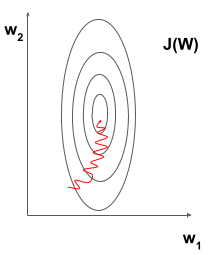
\includegraphics[width=0.3\linewidth]{imgs/featues-scaling-1}
    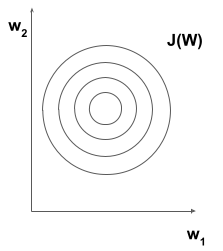
\includegraphics[width=0.3\linewidth]{imgs/scaling-2}
    \caption{Features scaling}
    \label{fig:scaling1}
\end{figure}

Cosi avremo una discesa del gradiente più regolare e meno suscettibile alle dimensioni
delle features.

\subsection{Feature scaling types}
\subsubsection{Min-Max normalizing}
\begin{equation}
    x' = \frac{x - min(x)}{max(x)-min(x)}
\end{equation}


\subsubsection{Mean normalizing}
\begin{equation}
    x'=\frac{x - average(x)}{max(x)-min(x)}
\end{equation}
\subsubsection{Standardizzation(or Z-score)}
\begin{equation}
    x'=\frac{x-average(x)}{\sigma}
\end{equation}
Dove sigma è la deviazion standard.

Ricordati che il preprocessing lo fai sul training, una volta ottenuto il tuo modello
per testarlo sul test, applica la standardizzation sul test e poi dallo al modello.

\subsection{Features selection}
\begin{itemize}
    \item alcune featires sono inutili
    \item se ho meno ridondanza, ho meno overfitting
    \item risualtato migliore
    \item meno tempo di training
\end{itemize}

\subsubsection{Univariate feature selection with chi2 test}
scegli le migliori featues usando chi2.
Questo risultato(chi2) può essere usato per selezionare le features.

Questo punteggio può essere usato per vedere quali features usare
in base al malore più alto del chi2 test, che deve avere solo valori positivi.

Il chi2 da un voto più alto alle features che sono più dipendenti con le altre
e un voto più basso alle features più indipendenti.


\subsubsection{Feature selection with Mutual information}
La mutua informazione(MI) è un numero alto se fra due variabili random
la dipendenza è alta.

Valore alto significa grande dipendenza.



Chi2 stima il grado di dipendenza lineare fra due variabili random, invece MI,
cattura ogni informazione inerente alla dipendenza statistica,
ma non essendo parametrizzabile, richiede più esempi per maggior precisione.

\subsection{Assunzioni sui dati}
\begin{itemize}
    \item un modello è una versione semplice del'osservazione, il semplificata significa che
    il modello scarta dettagli superflui che non sa generalizzare.
    Comunque, per decidere che dati scartare, devo fare \textbf{assunzioni}.
    \item Senza fare assunzioni sui dati, non c'è motivo di preferire un modello ad
    un'altro(\textbf{teoria del no più pranzo gratis})
    \begin{itemize}
        \item nessun modello funziona meglio a prescindere
        \item per capire quale modello è meglio faccio le prove e li valuto
        \item in alternativa alle prove, posso ragionare e fare assunzioni(linea guida generalissima)
        \begin{itemize}
            \item task semplici $\Rightarrow$ modello lineare con vari gradi di regolarizzazione
            \item task difficili $\Rightarrow$ reti neurali
        \end{itemize}
        \item attenzion al numer odi features rispetto al numero dei dati
    \end{itemize}
\end{itemize}

Un idea buona è di testare tanti modelli sui dati, ma questo porta ad un error
stocastico dei modelli e la divisione del dataset in test e train in maniera randomica.

Una soluzione potente è far fare tanti giri ad ogni signolo modello cosi  ta eliminare
il più possibile gli errori di natira stocastica.

minimo 10 giri suggeriti dal prof!

Una volta trovato l'algoritmo che fa meglio quel lavoro, si può fare
il \textbf{fine-tuning} degli hyper-parameters del modello.

\subsubsection{Come miglirare gli hyper-parameters}

Due modi principali:
\begin{itemize}
    \item Grid-search
    \begin{itemize}
        \item provare le combinaioni di preset e annotarsi i risultati
        \item quando ho finito le combinazioni, il modello viene fatto con le combinazioni di parametri migliori
        \item Il tempo pper valutare questo cresce in maniera esponenziale con l'aggiunta di parametri
    \end{itemize}
    \item random search
    \begin{itemize}
        \item si va a caso e si annotano i risulati con il tuning randomico fatto
        \item funziona con pochi dati
        \item è pprovato che il random è meglio empiricamente del grid
        \item se il dataset è grande, meglio usare in combo il random e il grid
    \end{itemize}
\end{itemize}


\subsection{K-fold cross-validation}
Se ho un data set piccolo uso questo trick,
divido il dataset in porzioni e a turno le do in pasto al modello(sempre per il discorso di fargli fare tanti giri).

\begin{figure}[H]
    \centering
    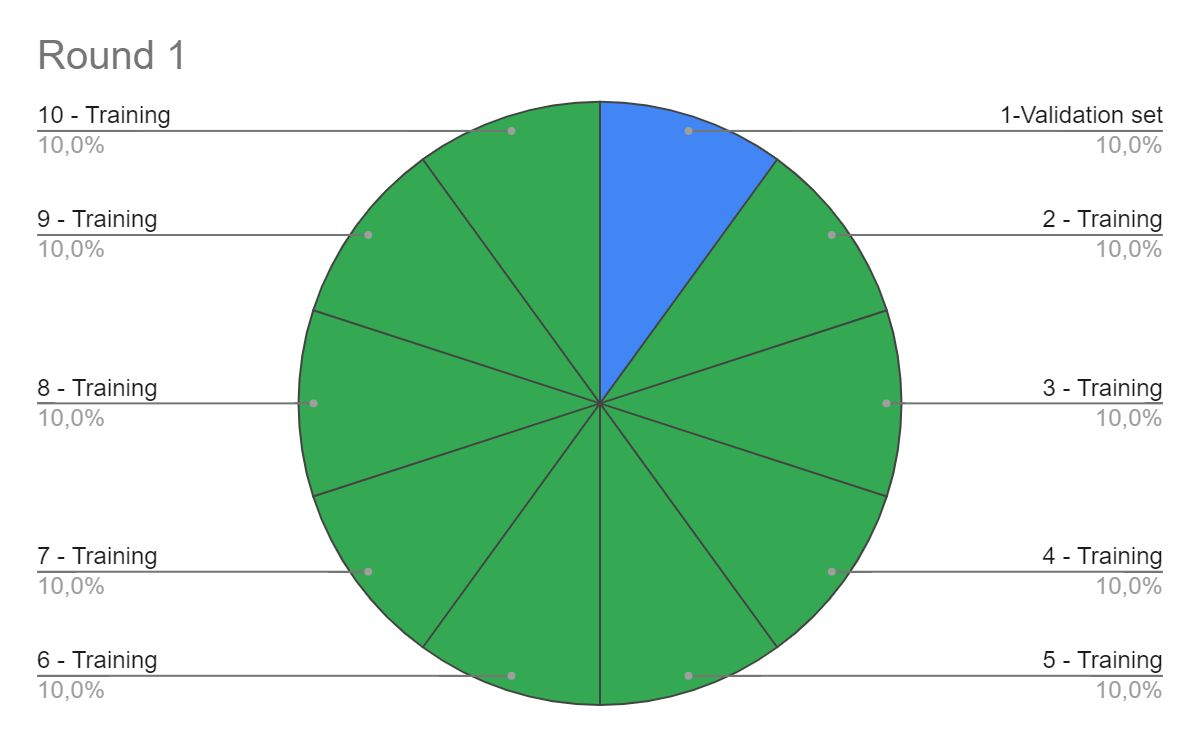
\includegraphics[width=0.6\linewidth]{imgs/k-fold}
    \caption{K-fold}
    \label{fig:kold}
\end{figure}


La cross validation permette di torvare oltre alla stima del modello,
ti permette acneh di capire quanto un modello è preciso.(tipo deviazione standard e altri)


\subsection{Riassunto della pipeline}
\begin{enumerate}
    \item Dividi il dataset in 80 training e 20 test
    \item applica il features scaling
    \item dal training estrai un 10 come validation(usa il validation per i test e il fine-tuning, se hai pochi dati usa il k-fold)
    \item crea un grid o un random search sui possibili parametri e valuta il modello con il validation set
    \item quando ha iun buon risultato, valuta il modello sul test setper vedere la generalizzazione
\end{enumerate}

\section{Unsupervised Learning}

I dati non hanno una label,
alcune task:
\begin{itemize}
    \item clustering
    \item dimensionality reduction
    \item anomaly detection
\end{itemize}

\subsection{Clustering}
Al sistema viene chiesto di raggruppare set di oggetti in gruppi(cluster), di modo
che gli oggetti di un gruppo siano parecchio simili.

Usato per trovare proprietà nascoste o irregolarità.

Anche il clustering è un problema di ottimizzazione, cerchiamo di raggruppare oggetti
in gruppi, entrano in gioco concetti come \textbf{variabilità(c)} e \textbf{dissimilarità}.

\begin{equation}
    variability(c_i) = \sum_{e\in c_i} distance(mean(c_i), e) ^2
\end{equation}

\begin{equation}
    dissimilarity(c) = \sum_{c_i\in c} variability(c_i)
\end{equation}

Per ottimizzare devo trovare dei cluster che minimizzino la dissimilarità con un numero
di cluster che decidiamo a priori(usare un cluster avrebbe dissimilarità bassa ma  non serve a
nulla).

I due metodi principali per il clustering sono: hierarchical clustering e K-Means.


\subsubsection{Hierarchical clustering(agglomerative clustering)}

\begin{enumerate}
    \item inizio con dare un cluster ad ogni oggetto(quindi ho un cluster per ogni oggetto e ogni claster contiene un oggetto)
    \item trova la coppia di cluster più simili e fai un merge
    \item ripeti fino ad ottenere un cluster di N item
\end{enumerate}

Trovare le coppie simili prende il nome di linking,
può essere singolo(semplice) o completo:
\begin{figure}[H]
    \centering
    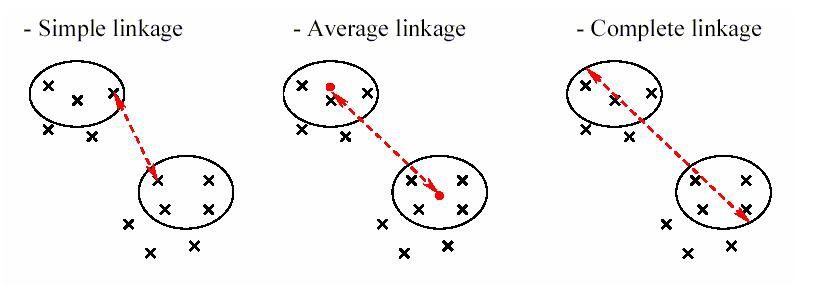
\includegraphics[width=0.6\linewidth]{imgs/linkag}
    \caption{Linkage}
    \label{fig:Linkage}
\end{figure}
\begin{itemize}
    \item simple linkage: la distanza fra cluster è tra i membri più vicini dei due cluster
    \item complete linkage: vede la distanza come la distanza massima possibile fra i due cluster
\end{itemize}


\begin{figure}[H]
    \centering
    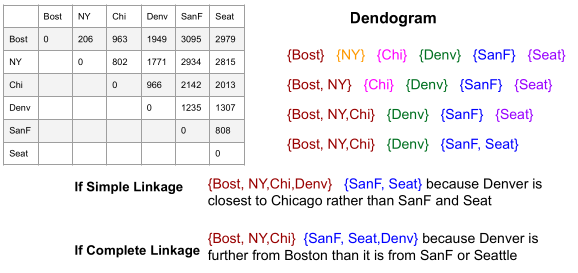
\includegraphics[width=0.6\linewidth]{imgs/esempio-clustering}
    \caption{Esempio clustering}
    \label{fig:Esempio-clustering}
\end{figure}


Nei cluster gerarchici:
\begin{itemize}
    \item il criterio di linking e deterministico(no random)
    \item il dendogramma è facilmete spiegabile
    \item è un algoritmo greedy
    \item è flessibile(cambia cirteri per differenti risultati)
    \item lento( complessità $O(N^3)$)
\end{itemize}


\subsubsection{K-Means}
\begin{itemize}
    \item Serve un algoritmo greedy più veloce
    \item k è il numero dei cluster che voglio
    \begin{enumerate}
        \item scegli un numero radom di centroidi k
        \item while true:
        \begin{enumerate}
            \item crea k cluster assegnando ogni esempio al centoride più vicino
            \item computa k nuovi centroidi facendo la media in ogni cluster
            \item se i centroidi non cambiano
            \begin{enumerate}
                \item fermati
            \end{enumerate}
        \end{enumerate}
    \end{enumerate}
\end{itemize}
\begin{figure}[H]
    \centering
    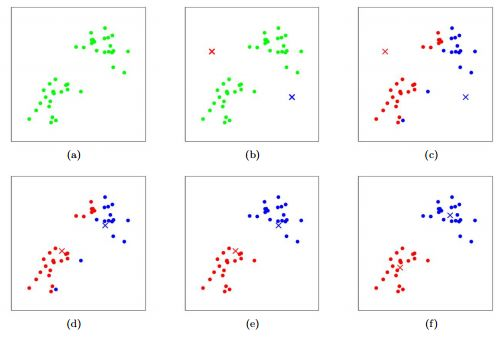
\includegraphics[width=0.8\linewidth]{/home/dmo/git/appunti-latex-2021-2022/Bid data e business intelligence/imgs/k-means}
    \caption{k-means}
    \label{fig:k-means}
\end{figure}


\subsection{La maledizione della dimensionalità}
È il problema che esce quando si danno ai modelli dati con multidimensionali.

Se si aggiungono tante features da prendere in considerazione, si possono separare
le classi in analisi ma lo spazio diventa enorme, se si usano troppe features,
si rischia di ottenere una separazione per ogni elemento del sistema.

Con l'aumento della dimensionalità lo spazio cresce e i daati saranno sempre più
sparsi.

\begin{figure}[H]
    \centering
    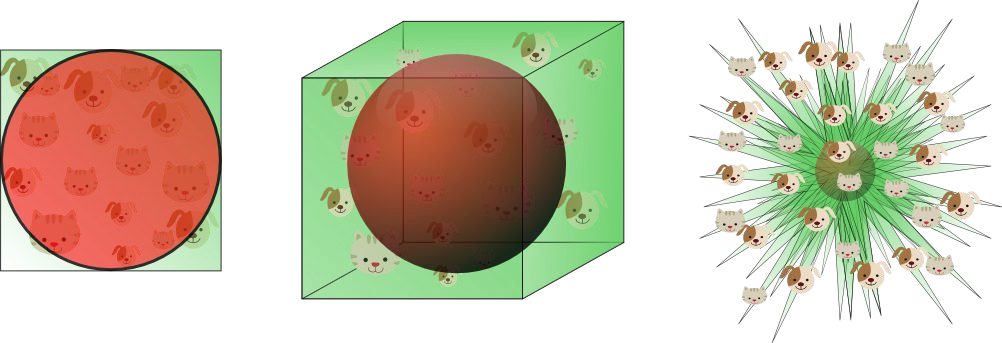
\includegraphics[width=0.6\linewidth]{imgs/curse-of-dimensionality}
    \caption{curse of dimensionality}
    \label{fig:curse_of_dimensionality}
\end{figure}
La quantità di dati richiesta da lproblema aumenta esponenzialmente con l'aumentare
della dimensionalità.

\subsection{Riduzione della dimensionalità}
Nei casi del mondo reale, i dati non sono sparsi nelle dimensioni in maniera uniforme,
alcune dimensioni sono costanti ecc.
La maggior parte delle istanze giace in un numero ristretto di dimensioni(o li vicino).


\subsubsection{Principal Component Analysis(PCA)}

PCA è l'algoritmo per la riduzione della dimensionalità più popolare.

\begin{itemize}
    \item identifica l'iperpiano che giace più vicino ai dati e li proietta su se stesso
    \item Per proiettare i dati su un iperpiano a dimensionalità minore, biogna trovare l'iperpiano giusto
    \begin{itemize}
        \item il miglio iperpiano è quello che conserva più dati
    \end{itemize}
\end{itemize}

\begin{figure}[H]
    \centering
    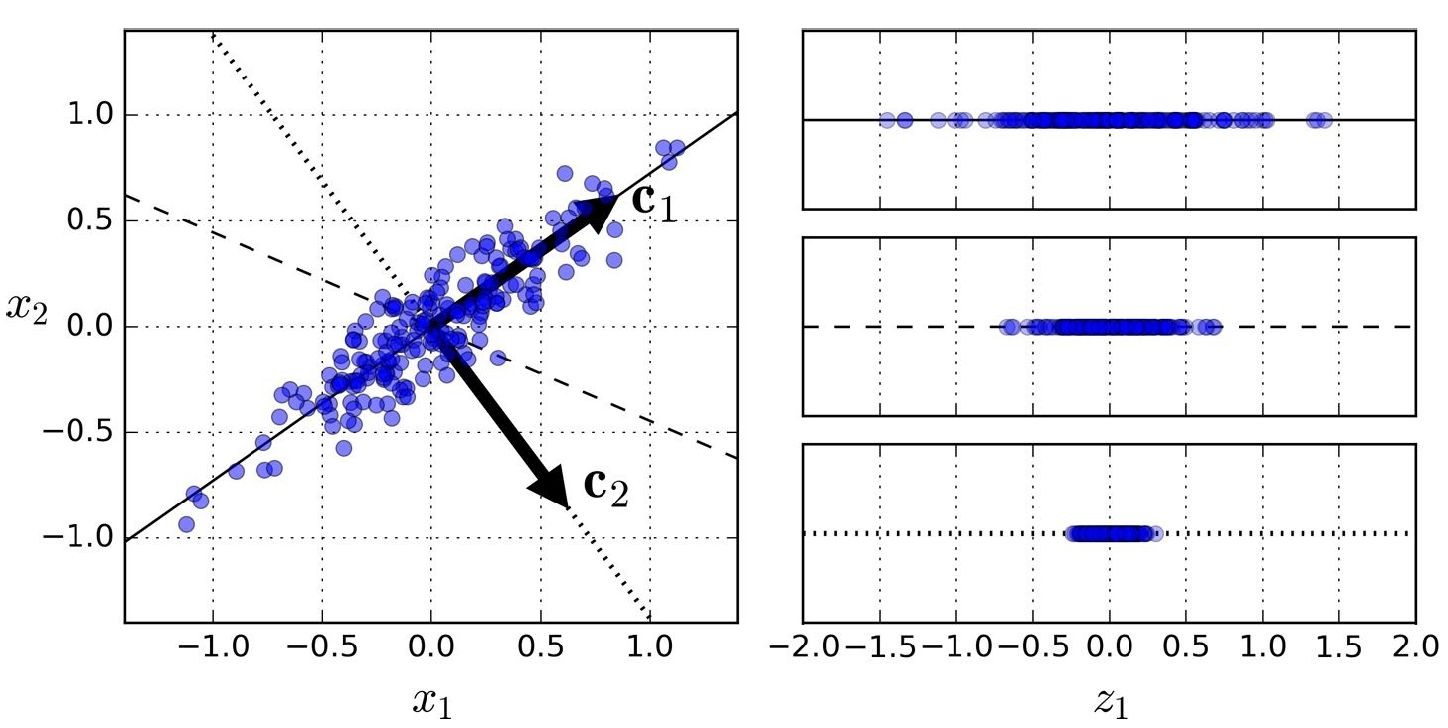
\includegraphics[width=0.5\linewidth]{/home/dmo/git/appunti-latex-2021-2022/Bid data e business intelligence/imgs/pca}
    \caption{PCA}
    \label{fig:PCA}
\end{figure}
PCA identifica l'asse che prende il maggior numero di variazioni(come nell'esempio),
in base a che dimensione vuoi raggiungere, calcola anche il secondo/terno asse ecc.
Se per esempio vuoi ridure a tre assi, ti troverà i tre assi dove collassano più dati.


L'iesimo asse è chiamato l'iesimo componente principale.

Un avolta identificati componenti principali, puoi ridurre le dimensioni.

\subsubsection{t-SNE}
t-distributed Stochastic Neighbor Embedding(t-SNE) è una tecnica di riduzione
dimensionale non lineare.

È lo stato dell'arte per gli algoritmo di riduzione di dimensioni per la data
visualizzation.


Modella ogni oggetto con tante dimensioni in modo che gli oggetti simili sono
modellati da punti vicini e oggetti non simili con punti lontani


\begin{itemize}
    \item SNE comincia con il convertire le distanze euclidee multi-dimensionali fra
    i dati in probabilità condizionali che rappresentano le similitudini.
    \item t-SNE costruisce una distribuzione di probabilità sulle coppie di oggetti con tante
    dimensioni di modo che oggetti simili abbiano una alt probabilità mentre gli oggetti
    meno simili probabilità minore
    \item t-SNE definisce una distribuzione di probabilità sui punti nella mappa a meno dimensioni
    e minimizza la Kullback-leibler divergence(KL-divergence) tra le due distribuzioni usando
    la discesa del gradiente.
    \item genera una spazio random e ci mette i dati randomicamente
    \item poi minimizza la discesa KL del gradiente in modo da preservare la vera distanza
    fra gli oggetti.
\end{itemize}



\subsubsection{recap t-SNE vs PCA}
\begin{itemize}
    \item t-SNE è iterativo non come PCA, non puoi applicarlo ad unaltro dataset come se niente fosse
    Con PCA una volta ottenuta la prima riduzione, si puo riapplicare ad altri dati
    \item PCA crea un sub spazio di quello originale che nel ML è una features importante.

    \item t-SNE è sconsigliato per il ML perchè crea uno spazio artificiale
    dove le features legate alla spazio possono essere meno informative
\end{itemize}






















